\section{Estimation} \label{sec:estimation}

\subsection{Naive non parametric estimation : the case of the variogram}
%\subsubsection{Naive estimators and their properties in the non informative selection case}
With the term \emph{naive estimation} we refer to the situation where the estimator does not take into account the mechanism selection. Therefore, in case of informative sampling, the estimator could suffer from selection bias.
A common approach to achieve a valid variogram estimator is composed by \emph{estimation} and \emph{fitting} of the variogram. In the former, an estimate of the variogram is obtained, while the latter phase is necessary since the estimators used in the first phase are usually not conditionally negative-definite.

Under the assumption of constant-mean, an estimator based on the method of moments is \citep{matheron1962traite}
\begin{equation*} \label{eq:variogram_hat}
2\hat{\gamma}\left(h\right)=\frac{1}{|N\left(h\right)|}\sum_{(\ell_1,\ell_2)\in N\left(h\right)}{\left(\Signal\left[\Sample[\ell_1]\right]-\Signal\left[\Sample[\ell_2]\right]\right)^{2}},\forall h\in\mathbb{R}^{d}
\end{equation*}

where $N\left(h\right)=\left\{\left(\ell_1,\ell_2\right)\in\{1,\ldots,\Samplesize\}^2:\Sample[\ell_1]-\Sample[\ell_2]=h\right\}$ and $|N\left(h\right)|$ is the number of distinct pairs in $N\left(h\right)$. 

\begin{property}
$E[N(h)\hat{\Semivariogram}(h)]=\Semivariogram(h)$
\end{property}


When data are irregularly spaced in $\mathbb{R}^{d}$, we can use
\begin{equation} \label{eq:variogram_hat1}
2\hat{\gamma}_{s}\left(h\left(l\right)\right)=\mathrm{average}\lbrace\left(\Signal\left[\Sample[\ell_1]\right]-\Signal\left[\Sample[\ell_2]\right]\right)^{2}:%\left(\Sample[\ell_1], \Sample[\ell_2]\right)\in N\left(h\right);
\|\Sample[\ell_1]-\Sample[\ell_2]\|\in[h\mp \alpha]\rbrace,
\end{equation}
where the tolerance $\alpha$ is a positive number.
%the region $T\left(h\left(l\right)\right)$ is a specified tolerance region in $\mathbb{R}^{d}$ around $h\left(l\right)$ $l=1,\dots,K$ {\color{red} Check variable $l$}.

%A robust version of \eqref{eq:variogram_hat} is given by \citep{cressie1980robust}
%\begin{equation} \label{eq:variogram_hat_robust}
%2\hat{\gamma}_{r}\left(h\right)=\Bigg\lbrace\frac{1}{|N\left(h\right)|}\sum_{N\left(h\right)}{|\Signal\left[\Sample[\ell_1]\right]-\Signal\left[\Sample[\ell_2]\right]|}^{1/2}\Bigg\rbrace ^{4}
%/ \left(0.457 + 0.494/|N\left(h\right)|\right)
%\end{equation} 
%and corresponding smoothed version
%\begin{equation}
%2\hat{\gamma}_{rs}=\left[med\lbrace|\Signal\left[\Sample[\ell_1]\right]-\Signal\left[\Sample[\ell_2]\right]|^{1/2}:\left(\Sample[\ell_1], \Sample[\ell_2]\right)\in N\left(h\right);h\in T\left(h\left(l\right)\right)\rbrace\right]^{4}/B\left(h\right)
%\end{equation}
%where $med$ is the median of the sequence and $B\left(h\right)$ is a correction-term for bias (asymptotically $B\left(h\right)=0.457$).

%A non-parametric approach to variogram estimation can be achieved by the use of kernel estimator
%\begin{equation}
%2\hat{\gamma}\left(h\right)=\frac{\sum_{i}\sum_{j}{w_{ij}\left(h\right)\left(\Signal\left[\Sample[\ell_1]\right]-\Signal\left[\Sample[\ell_2]\right]\right)^{2}}}{\sum_{i}\sum_{j}{w_{ij}\left(h\right)}}
%\end{equation}
%where $w_{ij}=K\left(\frac{h-||\Sample[\ell_1] - \Sample[\ell_2]||}{g}\right)$, $K$ is a symmetric, zero-mean (bounded) and $g$ is a positive number called bandwith.

%{\color{red}FP: I do not know if the following makes sense.} To sum up, we can write a general estimator form for the \emph{naive estimated variogram}
%\begin{equation} \label{eq:g_hat}
    %\hat{G}(h)=\sum_{ij\in\Sample}{\beta_{ij}(h)(\Signal\left[\Sample[\ell_1]\right]-\Signal\left[\Sample[\ell_2]\right])(\Signal\left[\Sample[\ell_1]\right]-\Signal\left[\Sample[\ell_2]\right])^{T}}
%\end{equation}
%where the term $\beta_{i,j}$ is a mapping that depends on the particular estimator used (and sample selected).

Once the estimated variogram is obtained (or \emph{empirical}), a model is fitted to it in order to achieve a valid variogram. At this stage, we are searching for a valid variogram ``closest'' to the empirical one, and typically we look into a subset of valid variograms $P=\lbrace2\gamma:2\gamma\left(\cdot\right)=2\gamma\left(\cdot;\parampop\right);\parampop\in\parampop\rbrace$. The best element of $P$ can be searched through several good-of-fitness criteria, such as maximum likelihood estimator or Least Squares method.

%Maximum Likelihood estimator relies heavily on Gaussian assumption, while Least Squares method requires few assumption about $Y\left(\position\right)$.
%The LS minimizing problem can be written as 
%\begin{equation*}
%min\lbrace\left(2\tilde{\gamma}-2\gamma\left(\parampop\right)\right)^{T}W^{-1}\left(\tilde{\gamma}-\gamma\left(\parampop\right)\right)
%\end{equation*}
%where $2\tilde{\gamma}$ is the empirical variogram, $2\gamma\left(\parampop\right)$ is a valid model variogram with the exact form known except the parameter $\parampop$, and $W$ is a weight matrix. If $W$ is an identity matrix, Ordinary Least Square criterion is employed; in case of $W=V$, with $V$ variance-covariance matrix, we have Generalized Least Square criterion, and if $V$ is diagonal, Weighted Least Square criterion is achieved.

In order to investigate the behaviour of the naive estimation, we carried out a Monte Carlo simulation. We simulated one replication of the same isotropic Gaussian process considered in the Example 1, that is $\Signal:\Omega\to(\Pop=[0,1]^2\to\mathbb{R})$, with $\forall \position\in\Pop$, $\mathrm{\mu}[\position]=0$ and with a Gaussian Covariogram with parameters $\parampop_1=5$, $\parampop_2=0.1$. Samples were selected by means of $\mathrm{bpp}(1, 100)$, $\mathrm{bpp}(\desvar_{1}, 100)$, and $\mathrm{bpp}(\desvar_{2}, 100)$, where  $\mathbf{\desvar}_{1}$ is generated with parameters $(\log(10)-(0.4^2+0.3^2),0,\sqrt{0.4^2+0.3^2})$, and $\mathbf{\desvar}_{2}$ is generated with parameters  $(\log(10)-(0.4^2+0.3^2),0.4,0.3)$, as in the Example 2.
The $\mathrm{bpp}(1, \samplesize)$ is by definition a non-informative sampling mechanism, while the $\mathrm{bpp}(\desvar, \samplesize)$ could introduce bias when the variable $\desvar$ is correlated with the signal $\signal$, as explained in the previous Sections. Note that $\desvar_{1}$ was generated independently from $\signal$ while $\desvar_{2}$ was generated dependently from $\signal$. Indeed, $\mathrm{cor}(\signal, \desvar_{1})\approx -0.08$ and $\mathrm{cor}(\signal, \desvar_{2})\approx 0.75$, where $\mathrm{cor}$ indicates the correlation between the two variables. For each sampling mechanism, $M=1,000$ samples were selected, and variograms estimated by the method of moments and fitted by the Weighted Least Square criterion. These estimated variograms are compared to the variogram obtained by using all the population values, which we call \emph{population variogram}. In the first row of Figure \ref{fig:sim_naive_est}, we compare the averages of the densities obtained by samples selected by means of the three different selection mechanisms. We note that when $\mathrm{bpp}(\desvar_{2}, 100)$ is employed, the average density is different from the \emph{population density}. In the second row of Figure \ref{fig:sim_naive_est}, we compare the expected value of the variograms obtained by the replications to the population variogram. The simulation shows that when the samples are selected by means of $\mathrm{bpp}(1, 100)$ and $\mathrm{bpp}(\desvar_{1}, 100)$, the Monte Carlo expected value of the sample variogram (indicated by the dotted line) is close to the population variogram (indicated by continuous line), while when the samples are selected by means of $\mathrm{bpp}(\desvar_{2}, 100)$, the Monte Carlo expected value of the sample variogram (indicated by the dotted line) is  different from the population variogram (continuous line). Therefore, bias is introduced by the selection mechanism.

\begin{figure}[H]
\caption{Naive estimation of the variogram. In the first row, average densities (dotted lines) are compared with the population density (continuous line). In the second row, expected values of the variogram (dotted lines) are compared with population variogram (continuous line).}
\centering
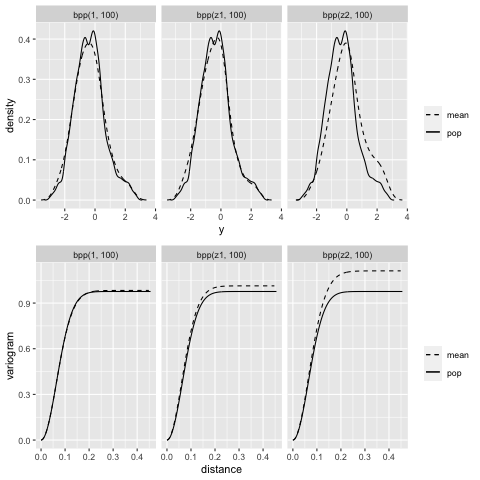
\includegraphics[width=0.7\textwidth]{fig/fig4.png}
\label{fig:sim_naive_est}
\end{figure}

%\begin{figure}[H]
%\caption{Relative Mean Squared Error to $\mathrm{bpp}(1, 100)$ of the variogram estimation}
%\label{fig:naive_est2}
%\centering
%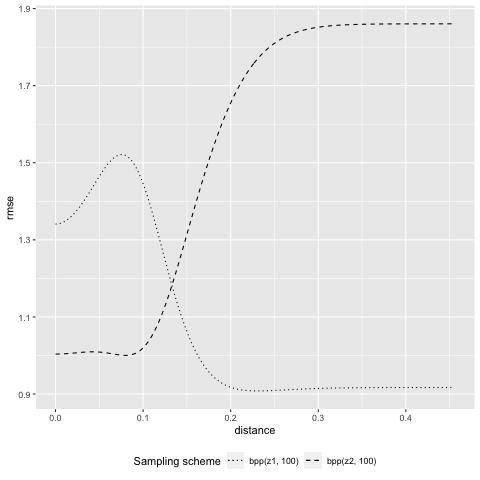
\includegraphics[width=0.6\textwidth]{fig/rmse.png}
%\end{figure}


\subsection{Maximum likelihood estimation}
%In particular, with ML we assume that the data $\Signal$ are multivariate Gaussian $(\textbf{X}\boldsymbol{\beta},{\color{red}\provar_{\position,\position^{'};\parampop}}$. The negative loglikelihood is {\color{red} FP: notation needs to be checked.} 
%{\color{red} DB: Can we just take the model with beta=0, Gaussian covariogram, $\parampop$ parameter of the covariogram (scale $\parampop_2$, and $\parampop_!=\sigma$).} 

%\begin{equation} \label{fit:ML}
%\likelihood\left(\boldsymbol{\beta},\parampop\right)=\left(n/2\right)\log{\left(2\pi\right)}+\left(1/2\right)\log{|\provar_{\position,\position^{'};\parampop}|}
%+\left(1/2\right)\left(\Signal-\textbf{X}\boldsymbol{\beta}\right)^{T}\provar_{\position,\position_{'};\parampop}^{-1}\left(\Signal-\textbf{X}\boldsymbol{\beta}\right)
%\end{equation}
%with estimators $\boldsymbol{\hat{\beta}}$ and $\hat{\parampop}$ satisfying $L\left(\boldsymbol{\hat{\beta}},\hat{\parampop}\right)=\inf{\lbrace L\left(\beta,\parampop\right):\boldsymbol{\beta}\in\mathbb{R}^{{\color{red}q}},\parampop\in\parampop\rbrace}$.

%\begin{equation} \label{fit:ML}
%\likelihood\left(\parampop\right)=\left(n/2\right)\log{\left(2\pi\right)}+\left(1/2\right)\log{|\provar_{\position,\position^{'};\parampop}|}
%+\left(1/2\right)\left(\Signal\right)^{T}\provar_{\position,\position_{'};\parampop}^{-1}\left(\Signal\right)
%\end{equation}
%with estimators $\hat{\parampop}$ satisfying $L(\hat{\parampop})=\inf{\lbrace L\left(\parampop\right):\parampop\in\parampop\rbrace}$.

Here we briefly present a possible solution that take into account the informativeness  of the sample. The proposal is based on the maximum likelihood estimation. In particular, in our setup, the loglikelihood of $\Signal[\position]$ is given by 

\begin{eqnarray} \label{Lnaive}
\likelihood_{\Signal[\position]}\left(\parampop;\signal\right)&=&\log(\density_{\Signal[\position]}(\signal;\parampop))\\&=&
\frac12\log{|\provar_{\position,\position^{'};\parampop}|}
+\frac12(\Signal[\Sample])^{\mathrm{T}}\provar_{\position,\position_{'};\parampop}^{-1}\Signal[\Sample]
\end{eqnarray}

and the naive estimator maximizes \eqref{Lnaive}. Indeed, this maximization ignores the selection mechanism. 

In order to take into account the informativeness of the sample, the \emph{full loglikelihood} should be used, which is composed by three factors: the density ratio, $\densityratio_{\Sample}(\position\mid\signal)$, the distribution of $\Signal$, $\density_{\Signal[\position]}(\signal)$, and the distribution of the sample, $\density_\Sample(\position)$. Therefore the loglikelihood is 

\begin{eqnarray} \label{fit:ML2}
\likelihood_{\Sample,\Signal[\Sample],\Samplesize}\left(\parampop,\paramnuisance;\position,\signal,\samplesize\right)&=&\log\left(\densityratio_{\Sample}(\position\mid\signal;\parampop,\paramnuisance)\right)+\log(\density_{\Signal[\position]}(\signal;\parampop))+\log\left(\density_\Sample(\position;\parampop,\paramnuisance)\right)
\end{eqnarray}

%{\color{red} Discuss here about what we do about $\density_\Sample(\position)$. Why we ignore it, although it may still contain information about $\theta$ and $\xi$, link to the debate about estimation in presence of nuisane parameters, reference to my draft paper and the approaches. Marginalisation or conditioning}


%REML estimators are obtained by applying maximum likelihood over error contrasts instead of the original data. %In the context of variogram estimation, the idea is to apply the likelihood over $\textbf{W}=\left(\Signal\left(1\right)-\Signal\left(2\right),\Signal\left(2\right)-\Signal\left(3\right),\dots,\Signal\left(n-1\right)-\Signal\left(n\right)\right)$
%Defining a vector of $n-\text{rank}\left(\Position\right)$ linearly independent (error) contrasts as $R=A^{T}\Signal$, where $A$ is an $\left(n-1\right)\times n$ matrix with elements
%\[
%a_{ij}=
%\begin{cases}
%1 &\text{for }i=j,j=1,\dots,n-1, \\
%-1&\text{for }i=j+1,j=1,\dots,n-1,\\
%0 &\text{elsewhere.}
%\end{cases}
%\]
%we have that $R\sim N\left(\textbf{0},A^{T}\provar_{\position,\position^{'};\parampop}A\right)$, which does not depend on $\boldsymbol{\beta}$. Moreover, if $A$ satisfies $AA^{T}=I-\Position\left(\Position^{T}\Position\right)^{-1}\Position^{T}$ and $A^{T}A=I$, we then have the following negative likelihood
%\begin{align*}
%L_{R}\left(\parampop\right)&=\left(\left(n-q\right)/2\right)\log{\left(2\pi\right)}-\left(1/2\right)\log{|\Position^{T}\Position|}+\left(1/2\right)\log{|\provar_{\position,\position^{'};\parampop}|}\\&+\left(1/2\right)\log{|\Position^{T}\provar_{\position,\position^{'};\parampop}^{-1}\Position |}+\left(1/2\right)\Signal^{T}\Pi\left(\parampop\right)\Signal
%\end{align*}
%where $\Pi\left(\parampop\right)=\provar_{\position,\position^{'};\parampop}^{-1}-\provar_{\position,\position^{'};\parampop}^{-1}\Position\left(\Position^{T}\provar_{\position,\position^{'};\parampop}^{-1}\Position\right)^{-1}\Position^{T}\provar_{\position,\position^{'};\parampop}^{-1}$ . Therefore, the REML estimate of $\parampop$ is obtained by minimizing $L_{R}\left(\parampop\right)$ over $\parampop$.




%Exact finite-sample distribution theory for estimators and corresponding variance estimators are available only in special circumstances (e.g. Jensen 1988). Therefore, simulations or approximation theory need to be employed in order to deal with intractable distribution theory. \cite{zimmerman1991comparison} presented a Monte Carlo comparison of different estimators, when two intrinsically stationary isotropic Gaussian random processes in $\mathbb{R}^{2}$ and various sampling intensities are taken into account. With regard to the MLE, different Authors agree that such approach can suffer from bias. \cite{warnes1987problems} illustrate potential problems by simulations of some simple spatial process, and \cite{mardia1989multimodality} indicate that these problems are caused by likelihoods not twice differentiable in $\parampop$. Moreover, a general conclusion that emerges from a set of several works based on simulations (Haining 1978c, Mardia and Meshall 1984, Swallow and Monahan 1984, Haining et al 1989, Zimmerman and Zimmerman 1991) is that the bias of MLE tends to be negative when the spatial dependence is positive, especially for small sample size. %{\color{red}and asymptotic variances of small-scale variation parameters are good approximation to exact variances only when the spatial dependence is weak.}

%For approximation theory, Cressie talks about two type of asymptotic theories {\color{red} pp }. \emph{Infill asympotics} refers to the the possibility to increase the sample size to infinity while the finite domain $D$ is kept fixed, whereas \emph{increase-domain asymptotics} refers to the situation where we take more units by means of increase the domain $D$. 

%Taken as it is from Cressie book (Section 7.3.1): when making inference on a random field $\lbrace Z(s):s\in D\rbrace$ from data $Z=(Z(s_{1},Z(s_{2}),\dots,Z(s_{n}))$, exact distribution theory of estimators, predictors, test statistics, and so on, is rarely available. Asymptotic distribution theory is the natural place to run for approximations, although, spatially, there are number of ways $n$ might tend to infinity.

%The \emph{naive estimated variogram} is 
%\begin{equation} \label{eq:g_hat}
    %\hat{G}(h)=\sum_{ij\in\Sample}{\beta_{ij}(h)(\Signal(\position_{i})-\Signal(\position_{j}))(\Signal(\position_{i})-Y(\position_{j}))^{T}}
%\end{equation}
%In equation \eqref{eq:g_hat}, the term $\beta_{i,j}$ is a mapping that may depend on the sample selected.
%Below we give possible definitions of $\beta_{i,j}$:
%\begin{equation}
    %\beta(\position_1,\position_2,h)=
    %\left|\begin{array}{l}
    %1 \text{ if } |\position_1-\position_2|=h, 0 \text{ otherwise}\\
    %\paramnuisance(\frac{|\position_{i}-\position_{j}|-h}{\alpha})
    %\end{array}\right.
%\end{equation},
%For binned estimation, a finite partition $(B_1,\ldots,B_n)$ of $\mathbb{R}^+$ is given as well as an element $h_k$ of each element $B_k$ of the partition. 
%Then the covariogram is first estimated for each $h_k$, as 
%...
%Then a covariogram is fitted 
%...
%In the following, we will not consider binned estimation.
%where {\color{red} $\paramnuisance$ is ..., and the bins $\mathrm{bin}_h=\left\{(i,j)\in\Sample^2\mid \left|\position_i-\position_j\right|\in [a_h,b_h)\right\}$}

%\subsection{Properties of the sample in the general case (including informative)}



 %Naive estimation of the population covariogram:
 %$E[naive~Covariogram]\neq$ pop cov,
 %$E[naive~Covariogram]=$ sample theoretical cov, 
 %with illustrative figures.




%\subsection{Parametric estimation}

